\section{Efficient KV Cache Reuse with RadixAttention}
\label{sec:radix_attention}


\lang programs can chain multiple generation calls and create parallel copies with the "\texttt{fork}" primitive.
Additionally, different program instances often share some common parts (e.g., system prompts). These scenarios create many shared prompt prefixes during execution, leading to numerous opportunities for reusing the KV cache.
During LLM inference, the KV cache stores intermediate tensors from the forward pass, reused for decoding future tokens. They are named after key-value pairs in the self-attention mechanism~\cite{vaswani2017attention}. KV cache computation depends only on prefix tokens. Therefore, requests with the same prompt prefix can reuse the KV cache, reducing redundant computation and memory usage. More background and some examples are provided in \autoref{sec:additional_radix_attention}.

Given the KV cache reuse opportunity, a key challenge in optimizing \lang programs is reusing the KV cache across multiple calls and instances. 
While some systems explore certain KV cache reuse cases~\cite{kwon2023vllm,ye2024chunkattention,juravsky2024hydragen,gim2023prompt}, they often need manual configurations and cannot handle all reuse patterns (e.g., dynamic tree structures). Consequently, most state-of-the-art inference systems recompute the KV cache for each request. We will discuss their limitations and our differences in \autoref{sec:related-work}.

This section introduces RadixAttention, a novel technique for automatic and systematic KV cache reuse during runtime. Unlike existing systems that discard the KV cache after a generation request finishes, our system retains the cache for prompts and generation results in a radix tree, enabling efficient prefix search, reuse, insertion, and eviction. We implement an LRU eviction policy and a cache-aware scheduling policy to enhance the cache hit rate. RadixAttention is compatible with techniques like continuous batching~\cite{yu2022orca}, paged attention~\cite{kwon2023vllm}, and tensor parallelism~\cite{shoeybi2019megatron}.
In addition, it introduces only negligible memory and time overhead when there is no cache hit.

\textbf{RadixAttention.}
A radix tree is a data structure that serves as a space-efficient alternative to a classical trie (prefix tree). Unlike typical trees, the edges of a radix tree can be labeled not just with single elements but also with sequences of elements of varying lengths, significantly enhancing efficiency.
In our system, we utilize a radix tree to manage a mapping between sequences of tokens, and their corresponding KV cache tensors. These KV cache tensors are stored in a non-contiguous, paged layout, where the size of each page is equivalent to one token.
Because GPU memory is quickly filled by the KV cahce, we introduce a simple LRU eviction policy that evicts the least recently used leaf first.  By evicting leaves first, we enable the re-use of their common ancestors until those ancestors become leaves and are also evicted.

In the continuous batching setting, we cannot evict nodes used by the currently running batch. Therefore, each node maintains a reference counter indicating how many running requests are using it. A node is evictable if its reference counter is zero. Note that we do not preallocate a fixed-size memory pool as a cache. Instead, we let the cached tokens and the currently running requests share the same memory pool. Therefore, the system dynamically allocates memory for cache and running requests. When enough waiting requests run, the system will evict all cached tokens in favor of a larger batch size.
\autoref{fig:example_radix_attn} shows how the radix tree is maintained for several incoming requests. 
The frontend interpreter sends full prompts to the runtime, and the runtime performs prefix matching and reuse. 
The tree structure is stored on the CPU with negligible maintenance overhead. 
During the execution of the \texttt{fork} primitive, the frontend sends the prefix first as a hint, ensuring the prefix is correctly inserted into the tree. It then sends the remaining prompts. This "Frontend Hint" simplifies runtime scheduling and matching, exemplifying the benefits of frontend-runtime co-design.


\begin{figure}[t]
\centering
\vspace{-2.5em}
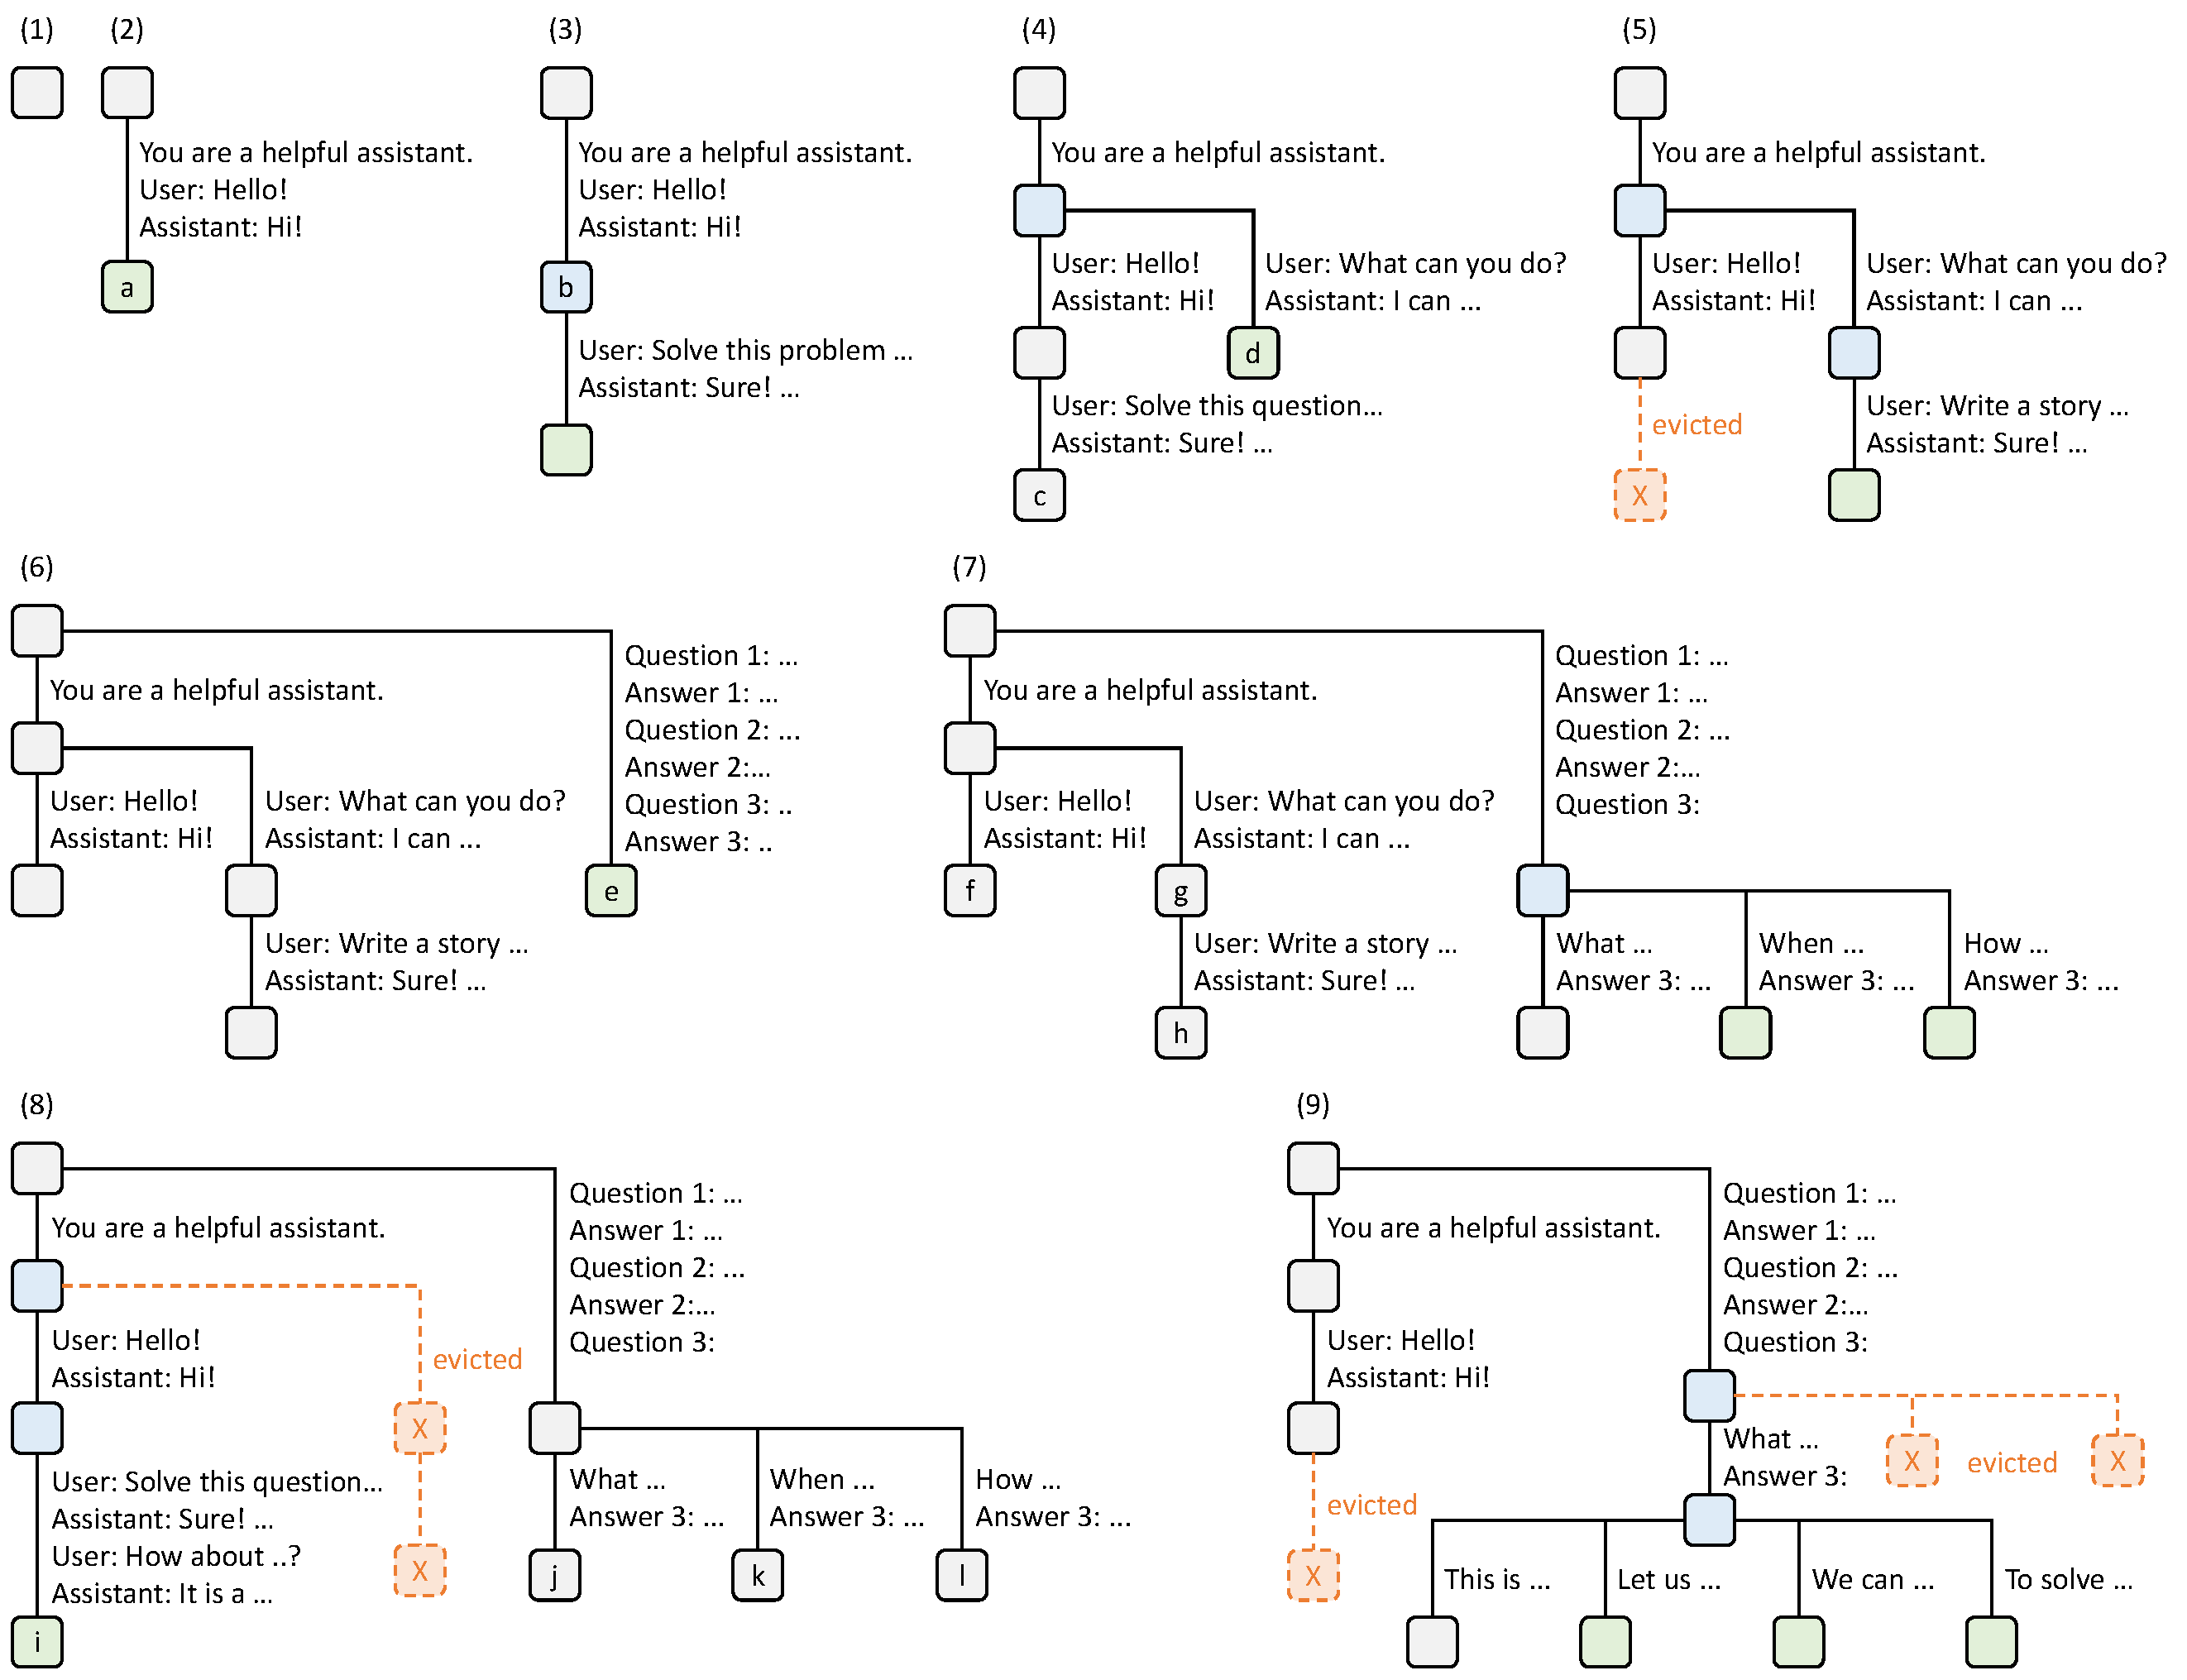
\includegraphics[width=0.99\linewidth]{figures/example_radix_attn.pdf}
\vspace{-0.5em}
\caption{
Examples of RadixAttention operations with an LRU eviction policy, illustrated across nine time points.
The figure demonstrates the dynamic evolution of the radix tree in response to various requests. These requests include two chat sessions, a batch of few-shot learning inquiries, and a self-consistency sampling.
Each tree edge carries a label denoting a substring or a sequence of tokens. The nodes are color-coded to reflect different states: green for newly added nodes, blue for cached nodes accessed during the time point, and red for nodes that have been evicted.
In step (1), the radix tree is initially empty.
In step (2), the server processes an incoming user message "Hello" and responds with the LLM output "Hi". The system prompt "You are a helpful assistant", the user message "Hello!", and the LLM reply "Hi!" are consolidated into the tree as a single edge linked to a new node.
In step (3), a new prompt arrives and the server finds the prefix of the prompt (i.e., the first turn of the conversation) in the radix tree and reuses its KV cache. The new turn is appended to the tree as a new node.
In step (4), a new chat session begins. The node ``b'' from (3) is split into two nodes to allow the two chat sessions to share the system prompt.
In step (5), the second chat session continues. However, due to the memory limit, node "c" from (4) must be evicted. The new turn is appended after node "d" in (4).
In step (6), the server receives a few-shot learning query, processes it, and inserts it into the tree. The root node is split because the new query does not share any prefix with existing nodes.
In step (7), the server receives a batch of additional few-shot learning queries. These queries share the same set of few-shot examples, so we split node 'e' from (6) to enable sharing.
In step (8), the server receives a new message from the first chat session. It evicts all nodes from the second chat session (node "g" and "h") as they are least recently used.
In step (9), the server receives a request to sample more answers for the questions in node "j" from (8), likely for self-consistency prompting. To make space for these requests, we evict node "i", "k", and "l" in (8).
}
\vspace{-1em}
\label{fig:example_radix_attn}
\end{figure}

\textbf{Cache-aware scheduling.}
We define the cache hit rate as $\frac{\text{number of cached prompt tokens}}{\text{number of prompt tokens}}$. 
When there are many requests in the waiting queue, the order in which they are executed can significantly impact the cache hit rate. For example, if the request scheduler frequently switches between different, unrelated requests, it can lead to cache thrashing and a low hit rate.
We design a cache-aware scheduling algorithm to increase the cache hit rate. 
In the batch-processing setting we
sort the requests by matched prefix length and prioritize requests with longer matched prefixes instead of using a first-come, first-served schedule. \autoref{alg:cache_aware_scheduling} (Appendix) shows the pseudo-code for cache-aware scheduling with contiguous batching. The algorithm uses longest-shared-prefix-first order.
In more latency-sensitive settings we may still be able to tolerate limited batch re-ordering to improve cache reuse. 
Additionally, we prove the following theorem for optimal scheduling in the offline case.
\footnote{In practice, the computation is not the same as what is described in the proof of \autoref{thm:optimal} because the unpredictable number of output tokens can cause the recomputation of the KV cache.}

\vspace{-0.2em}
\begin{restatable}{theorem}{optimal}
\label{thm:optimal}
For a batch of requests, we can achieve an optimal cache hit rate by visiting the radix tree of the requests in the depth-first search order, with a cache size $\geq$ the maximum request length. The longest-shared-prefix-first order is equivalent to a depth-first search order.
\end{restatable}
\vspace{-0.2em}

The proof is in \autoref{subsec:schedule_proof} (Appendix).
In the online case, the DFS order will be disrupted, but our schedule still approximates the DFS behavior on the augmented part of the full radix tree, as described in \autoref{subsec:schedule_proof}.
While greedy cache-aware scheduling can achieve high throughput, it can lead to starvation. We leave its integration with other fair scheduling methods~\cite{sheng2023fairness} as future work.

\textbf{Distributed Cases.} RadixAttention can be extended to multiple GPUs. For tensor parallelism, each GPU maintains a sharded KV cache. There is no need for additional synchronization because the tree operations are the same.
Data parallelism with multiple workers is discussed in \autoref{subsec:distributed_radix_attention} (Appendix).















